\documentclass{amsart}
\usepackage{harvard}
\newcommand{\Robject}[1]{{\texttt{#1}}}
\newcommand{\Rfunction}[1]{{\texttt{#1}}}
\newcommand{\Rpackage}[1]{{\texttt{#1}}}
\newcommand{\Rclass}[1]{{\textit{#1}}}
\newcommand{\Rmethod}[1]{{\textit{#1}}}
\newcommand{\Rfunarg}[1]{{\textit{#1}}}
\newcommand{\R}{{\normalfont\textsf{R }}{}}
\renewcommand{\S}{{\normalfont\textsf{S }}{}}

\title{IRT in R - Vignette}
\thanks{Version:  \today}
\author{}

\usepackage{/Library/Frameworks/R.framework/Versions/2.7/Resources/share/texmf/Sweave}
\begin{document}
\bibliographystyle{econometrica}
\begin{abstract}
	umes that the outcome is a probabilistic function of a single latent
	trait; the distribution of this trait varies across the population
	and it is informative to condition this distribution on covariates.
	The responses of those with higher values of the trait first--order
	stochastically dominate the response of those with lower values of
	the trait.\\
Vignette presents a brief introduction to the \Rpackage{irt} package written in \R language.
Both \R and \Rpackage{irt} are open-source software projects.
\Rpackage{irt} can be downloaded from \texttt{http://code.google.com/p/rsirt/downloads/list}.\\
(Thanks to Mayssun, Konrad, Anna.)
\end{abstract}

\maketitle

\pagestyle{myheadings}
\markboth{\sc \Rpackage{irt} in \R}{\sc}

%--------------------------------------------------------
\section{This document }
While writing this document we follow Sweave formatting of \citeasnoun{Leisch} which is an implementation 
of the literate programming style initiated by \citeasnoun{Knuth.LP}. It allows for interplay between code, output and comments...\\

\emph{irt()} is not particularly fast or efficient and the problem
is highly nonlinear; Because of the highly nonlinear nature of the problem, default values
of the convergence parameters are set to very tight tolerances. The
warning messages such as: 

...

are harmless.
%--------------------------------------------------------

\section{Introduction}
There is a response $r$ that is ordered and discrete and a latent
trait or factor $\theta$ whose value determines te probability distribution
of $r$. The possible outcomes for $r$ will be labelled $1,2,3,...$
where higher values of the outcome are `more common' for higher values
of $\theta.$ Specifically, if $\theta_{2}>\theta_{1}$ then the responses
of the $\theta_{2}$ population will stochastically dominate the responses
of the $\theta_{1}$ population. This corresponds to a notion that
more of $\theta$ leads to more of the response.

In the context at hand, there are $i=1,...,n$ individuals who are
have characteristics $W_{i}.$ These characteristics are assumed to
have no effect on $r$ except through $\theta.$ We embody this assumption
by writing\begin{equation}
p(r|W)=\int p(r|\theta)f(\theta|W)d\theta\label{eq1}\end{equation}
We wish to estimate both $p(r|\theta)$ and $f(\theta|W)$ with as
few assumptions as possible.

We start by observing that if $\theta$ were observable, we could
rescale it (i.e. apply a strictly monotonic transformation to it)
and, provided we adjusted $p(r|\theta)$ appropriately, $p(r|W)$
would remain unchanged, as would all the essential features of the
problem. Since here $\theta$ is not directly observed, we can choose
to `scale' it for the population or a specific sub-population. So
we could for example, say that the entire population is characterized
by $\theta$ being standard uniform or normal. An alternative, which
we adopt here, is to designate standard characteristic $W^{s}$ such
that $f\left(\theta|W^{s}\right)$ is a `standard' distribution---either
standard normal or standard uniform as taste and convenience dictate.

%------------------------------------------------------------------
\section{ Specification of $p(r|\theta)$ }

In the example to follow there are 4 responses (answers to an attitudinal
question or \char`\"{}item\char`\"{}) so we need to specify $F(r=3|\theta),$
$F(r=2|\theta),$ and $F(r=1|\theta),$ which correspond to the probabilities,
respectively, of answering \char`\"{}3\char`\"{} or less, \char`\"{}2\char`\"{}
or less, and \char`\"{}1\char`\"{}. Thus the probability of answering
\char`\"{}2\char`\"{} is $F(r=2|\theta)-$ $F(r=1|\theta).$ Stochastic
dominance requires e.g. $F(r=2|\theta_{2})<F(r=2|\theta_{1})$ if
$\theta_{2}>\theta_{1}.$ Graphing the four estimated $F(r|\theta)$
curves as function of $\theta$ with $\theta$ measured on $(0,1)$
yields:

When $\theta$ is measured on (0,1) (so e.g. $U(0,1)$ for $W=W^{s}),$
we seek a function that is \emph{downward} sloping in $\theta$ for
each $F(r|\theta),$ and which takes $(0,1)$ into $(0,1).$ There
is no particular harm (in the sense of implicitly imposing a substantive
restriction) if we take this function to be continuous. So a candidate
for $F(r=i|\theta)$ is $1-G_{i}(\theta),$ where $G_{i}()$ is a
distribution function on $(0,1).$ (Remember: $F(r|\theta)$ is a
discrete distribution function \emph{in r} for each value of $\theta.$)
How shall $G_{i}(\theta)$ be constructed? The stochastic dominance
conditions in $\theta$ require that the curves show in Figure 1 be
downward sloping and not cross.

irt1() constructs $G_{i}(\theta)$ as the distribution function corresponding
to an exponential tilt of the uniform density. Thus \[
G_{i}(\theta)=\frac{\int_{0}^{\theta}e^{_{1}t_{1}\gamma_{1}(u)+t_{2}\gamma_{2}(u)+...t_{m}\gamma_{m}(u)}du}{\int_{0}^{1}e^{t_{1}\gamma_{1}(u)+t_{2}\gamma_{2}(u)+...t_{m}\gamma_{m}(u)}du},\]
where the functions $\gamma_{1}(u),\gamma_{2}(u),...,\gamma_{m}(u)$
are $m$ basis functions, here chosen to be the (shifted) Legendre
polynomials. (Using these is equivalent to using a polynomial basis
but numerically more stable.)

We now turn to the problem of enforcing stochastic dominance. If there
are $k$ (ordered) responses, $F(k|\theta)=1$ by definition. Suppose
we are given a (distribution) function $G_{k-1}(\theta)$ and we construct
$F(k-1|\theta)$ as $1-G_{k-1}(\theta).$ An arbitrary $G_{k-2}(\theta)$
used in the same way---i.e. to define $F(k-2|\theta)=1-G_{k-2}(\theta)$---
will not in general lie below $F(k-1|\theta).$ But $F(k-2|\theta)$
constructed as $F(k-2|\theta)=[1-G_{k-2}(\theta)]F(k-1|\theta)$ will
have the required properties. In addition, it will enforce stochastic
dominance in hazard order, which is desirable; this is discussed below.
So we will construct $F(k-2|\theta)....F(1|\theta)$ in this fashion.

Once this is done, the probability of the response \char`\"{}$k$\char`\"{}
is given by $p(k|\theta)=1-F(k-1|\theta);$ $p(k-1|\theta)=$ $F(k-1|\theta)-F(k-2|\theta);$
etc., with $p(1|\theta)=F(1|\theta).$

\section{Specification of $f(\theta|W)$ }

Whereas irt1() attempts to be semiparametric about $p(r|\theta)$,
it is unabashedly parametric concerning $f(\theta|W).$ In applications,
$W$ consists largely of categorical values, so that a standard value
of $W,$ denoted $W^{s}$, is given by the characteristics which correspond
to 0 for all the categorical (or \char`\"{}dummy\char`\"{}) variables.
When there is a continuous or pseudo--continuous variable (\emph{age}
and \emph{age}$^{2}$ in the example to follow), it is natural to
rescale the variable so it takes the value zero at e.g. the mean of
the sample. Consequently irt1() models $\theta$ as $N(W\delta,1),$
that is, to have a normal distribution with mean $W\delta$ and standard
deviation 1. When $W^{s}$ is defined so $W^{s}=0,$ (there is no
intercept included in $W)$ then $f(\theta|W^{s})$ is $N(0,1).$

It is possible to make this specification more flexible by allowing
$f(\theta|W)$ to have a variance that varies with $W;$ $f(\theta|W)\sim N(W\delta,$
$\sigma^{2}(W))$ with $\log\sigma=W\gamma$ is one possibility we
have pursued in other work. It is not implemented here.

Modeling $\theta$ on a `normal' scale ostensibly conflicts with the
construction of $p(r|\theta)$ above (embodied in Figure 1), which
was done on a $(0,1)$ scale. The curves displayed in Figure 1 are
indeed just curves (they are not themselves probability distributions,
but a display of the relation between probability distributions),
so by applying any inverse distribution function with range $(-\infty,\infty)$
we can \char`\"{}stretch\char`\"{} these curves appropriately. Applying
the inverse standard normal distribution to Figure 1's curves gives:

%------------------------------------------------------------------
\section{The Mechanics of irt1()} 

\Rpackage{irt} is an \R package to estimate the model of equation (...)
by maximum likelihood; the integration is carried out by a Gauss--Legendre
quadrature.

\Rpackage{irt} is distributed together with an extract of data from the 2002
Pew Survey of American adults (see Spady cemmap papers for some documentation.)
The data of 2502 observations (call {\tt data(elections)}) has variables which can be described in 4 categories:

\begin{itemize}
\item (CITEMS) 4 category responses to 7 `cultural' items. 
These are coded so that `4' is the most `liberal' response.\\
These are: {\it unborn,womentradrole,peacethrustrength
 searchterrorists, bandangerousbooks, firegayteachers, xratedOK}

\item (EITEMS) 4 category responses to 7 `cultural' items.  
These are coded so that `4' is the most `liberal' response.\\
These are: {\it govguareatsleep, govtakecarewhocant,govhelpneedy, improveblackpos,equalOPP,poortoodep,       
richgetricher,govwasteful}
\item (VOTE) respondents' report of how they voted
in the 2000 Presidential election: Bush, Gore, Other, Did not vote.
Other is primarily Nader. Unlike other Pew surveys, the 2002 survey
does \emph{not} give vote proportions in accord with the popular vote;
Bush is overrepresented.\\
These are: {\it bush,gore,other,novote}

\item (Wx) demographic characteristics. `age' is centered at about 45.8 and
agesq.01 is $(yrs-45.8)^{2}/100$
These are: ....
\end{itemize}


%--------------------------------------------------------
\section{Getting Started}
To install \Rpackage{irt} do .... \\

Once \Rpackage{irt} installed load it to the \R session
\begin{Schunk}
\begin{Sinput}
> library(irt)
\end{Sinput}
\end{Schunk}

Help for \Rpackage{irt} can be found by writing in \R 
\begin{Schunk}
\begin{Sinput}
> help(package = "irt")
> help(irt)
\end{Sinput}
\end{Schunk}
An convenient shorthand for the latter command is to type simply
\texttt{?rq}.\\

They do following ....


%--------------------------------------------------------
\newpage
\section{Basics of \Rpackage{irt}}
There are four basic steps to conduct IRT estimation with \Rpackage{irt} package
\begin{enumerate}
	\item upload and manipulate a data set
	\item construct an item
	\item run irt estimations
	\item summarize results
\end{enumerate}
While the first and the last step are standard in any data analysis, construction of item and estimation procedure
are typical for \Rpackage{irt} package. We start with very simple example based on {\tt elections} data set (describe data set)
from \Rpackage{irt} package. \\
First we load a package, data set and look up at variables.

\begin{Schunk}
\begin{Sinput}
> library(irt)
> data(elections)
> print(names(elections))
\end{Sinput}
\begin{Soutput}
 [1] "govguareatsleep"    "govtakecarewhocant"
 [3] "govhelpneedy"       "improveblackpos"   
 [5] "equalOPP"           "poortoodep"        
 [7] "richgetricher"      "govwasteful"       
 [9] "age"                "agesq.01"          
[11] "black"              "bornagain"         
[13] "blackbornagain"     "rel.catholic"      
[15] "rel.nonchr"         "ed.cat1"           
[17] "ed.cat3"            "ed.cat4"           
[19] "ed.cat5"            "income.1"          
[21] "income.3"           "income.4"          
[23] "income.dk"          "parent"            
[25] "hispanic"           "female"            
\end{Soutput}
\end{Schunk}
Now we construct an items matrix and design matrix (we do it for consistency with rhs examples).

\begin{Schunk}
\begin{Sinput}
> EITEMS <- elections[, 1:8]
> W <- elections[, 9:26]
\end{Sinput}
\end{Schunk}
at this point we are ready to work with items constructors. First we consider single item model for {\it govguareatsleep}.
We use a function {\tt item()} to construct a single item as follows:
\begin{Schunk}
\begin{Sinput}
> singleItem <- item(EITEMS[, 1], W, itemnm = "govguareatsleep")
\end{Sinput}
\end{Schunk}
We input optional {\tt itemnm} to force the name of the item. Having an item we can run irt and summarize results.

\begin{Schunk}
\begin{Sinput}
> res <- irt(singleItem)
> print(res)
> summary(res)
\end{Sinput}
\end{Schunk}
It is important to note that function {\tt summary} computes jacobian and hessian matrix which may take some time.\\
We can also summarize the result on a plot.
\begin{figure}[hptb] 
\begin{center}
{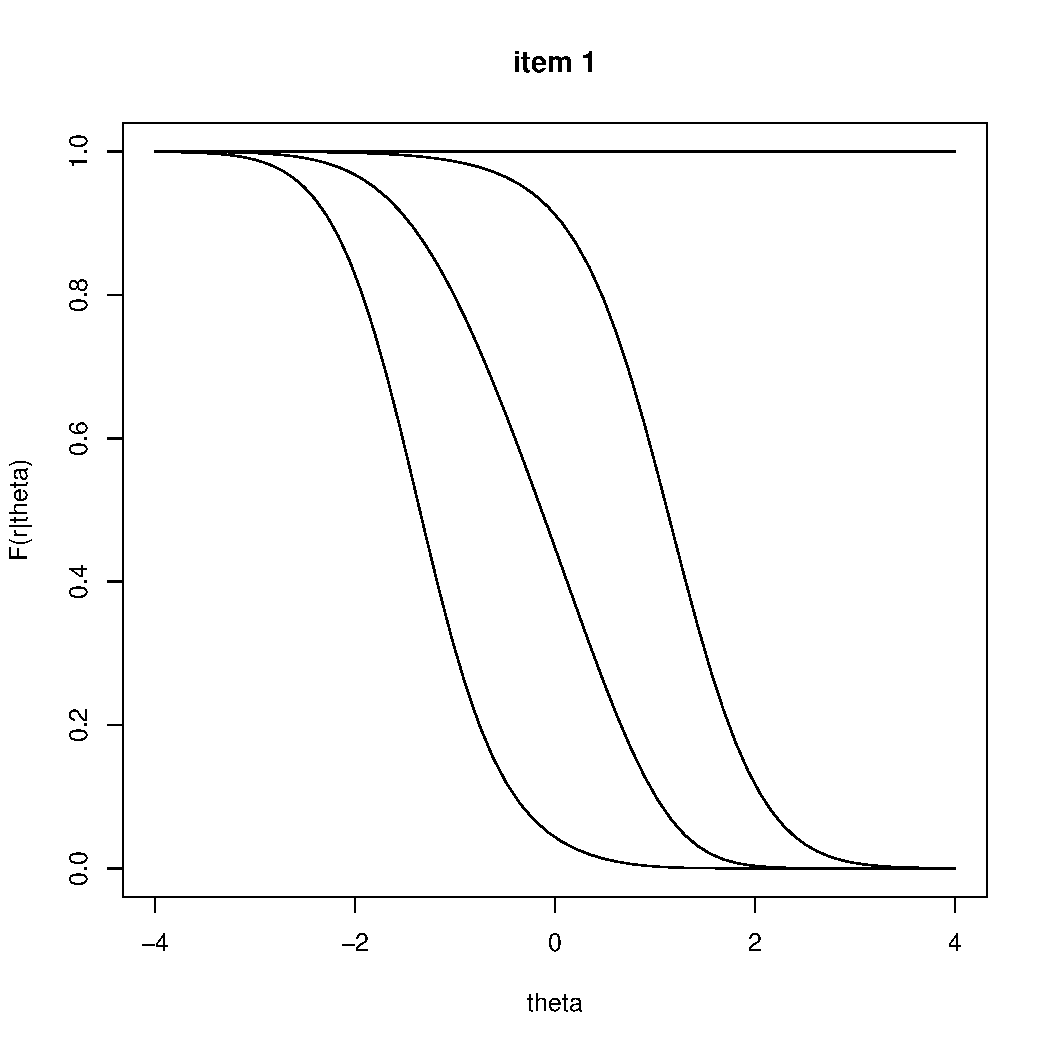
\includegraphics[width=6cm]{./graph/singleItemPltStd.pdf}}
\end{center}
\caption{Standard irt plot.}
\end{figure}
\newpage
%--------------------------------------------------------
\section{Single Item Model}
Single item model ...
\begin{Schunk}
\begin{Sinput}
> library(irt)
> data(elections)
> attach(elections)
> W <- cbind(age, agesq.01, black, bornagain, blackbornagain, 
+     rel.catholic, rel.nonchr)
> singleItem <- item(govguareatsleep, W)
> res <- irt(singleItem)
> detach(elections)
\end{Sinput}
\end{Schunk}
%--------------------------------------------------------
\section{Single Item Model - formula mode}

Single item model has a formula mode for item constructor. Note that we do not need to attach data. Data set enters as an input to item constructor.

\begin{Schunk}
\begin{Sinput}
> data(elections)
> singleItem <- item(govguareatsleep ~ age + agesq.01 + 
+     black, ~black, data = elections)
> res <- irt(singleItem)
\end{Sinput}
\end{Schunk}
%--------------------------------------------------------
\section{Multiple Items Model}
Multiple items model differs from single items model by items constructor. Construction of an item is done by {\tt multipleitem()} function and the model can be run as follows

\begin{Schunk}
\begin{Sinput}
> library(irt)
> data(elections)
> attach(elections)
> EITEMS <- cbind(govguareatsleep, govtakecarewhocant, 
+     govhelpneedy)
> W <- elections[, 9:26]
> items <- multipleitem(EITEMS, W)
> res <- irt(items, iSet = iSet)
> detach(elections)
\end{Sinput}
\end{Schunk}
This is four items model.
%--------------------------------------------------------
\section{IRT optimization settings}
Package \Rpackage{irt} contains a class {\tt irtSet} which constitutes a basis
for optimization. We can look up its default options as follows
\begin{Schunk}
\begin{Sinput}
> iSet <- irtSet()
> print(iSet)
\end{Sinput}
\begin{Soutput}
 Basic settings for irt optimization:
 ======================================== 
        algorithm : nlm
          Fmethod : ET
            ctype : F
               nb : 2
          gradtol : 1e-11
           reltol : 1e-09
          iterlim : 250
               pl : 2
              tag : 2008-08-08-run25
            bfile : bbest.2008-08-08-run25
       orthobasis : TRUE
\end{Soutput}
\end{Schunk}
Output of irtSet() is a list of optimization options. These options determine behavior of the estimator.
They can be modified on the initial call.

\begin{Schunk}
\begin{Sinput}
> iSet <- irtSet(iterlim = 10, pl = 0, tag = "mymModel", 
+     orthobasis = FALSE)
> print(iSet)
\end{Sinput}
\begin{Soutput}
 Basic settings for irt optimization:
 ======================================== 
        algorithm : nlm
          Fmethod : ET
            ctype : F
               nb : 2
          gradtol : 1e-11
           reltol : 1e-09
          iterlim : 10
               pl : 0
              tag : mymModel
            bfile : bbest.mymModel
       orthobasis : FALSE
\end{Soutput}
\end{Schunk}
Modified settings can be passed to {\tt irt()} function through {\tt iSet} option. Therefore the total run of a single item model would be 
\begin{Schunk}
\begin{Sinput}
> data(elections)
> iSet <- irtSet(iterlim = 50, pl = 0, tag = "myModel")
> singleItem <- item(govguareatsleep ~ age + agesq.01 + 
+     black, ~black, data = elections, iSet = iSet)
> res <- irt(singleItem)
\end{Sinput}
\end{Schunk}
In the same fashion we do it for multiple items model.

%--------------------------------------------------------
\newpage
\section{Plotting Methods}
Package has advanced plotting method. They are implemented in a standard \R plotting framework as well as {\tt grid} graphics model. Box-Plot model is saved in the {\tt Ftab} in the output from {\tt irt()}. It is of the class {\tt Ftab}. Generic method {\tt plot}  operates in this class of objects. 

\begin{Schunk}
\begin{Sinput}
> Ftab <- res$Fab
> plot(Ftab)
\end{Sinput}
\end{Schunk}
This produces standard plot with default options

%\begin{figure}[hptb] 
\begin{center}
{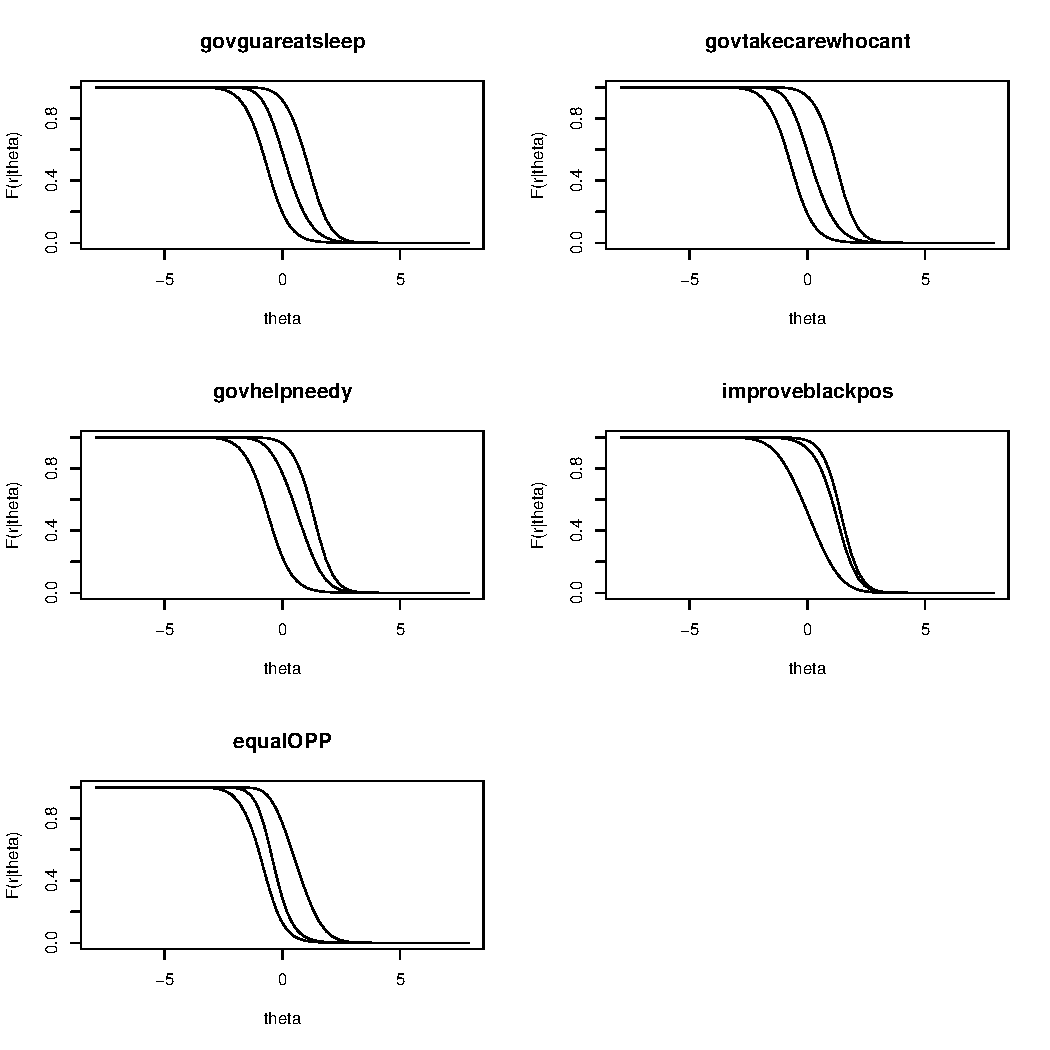
\includegraphics[width=12cm]{./graph/plotStd1.pdf}}
\end{center}
%\caption{Standard irt plot.}
%\end{figure}

We can rescale this figure setting xscale option

\begin{Schunk}
\begin{Sinput}
> plot(Ftab, xscale = c(-2, 2))
\end{Sinput}
\end{Schunk}

%\begin{figure}[hptb] 
\begin{center}
{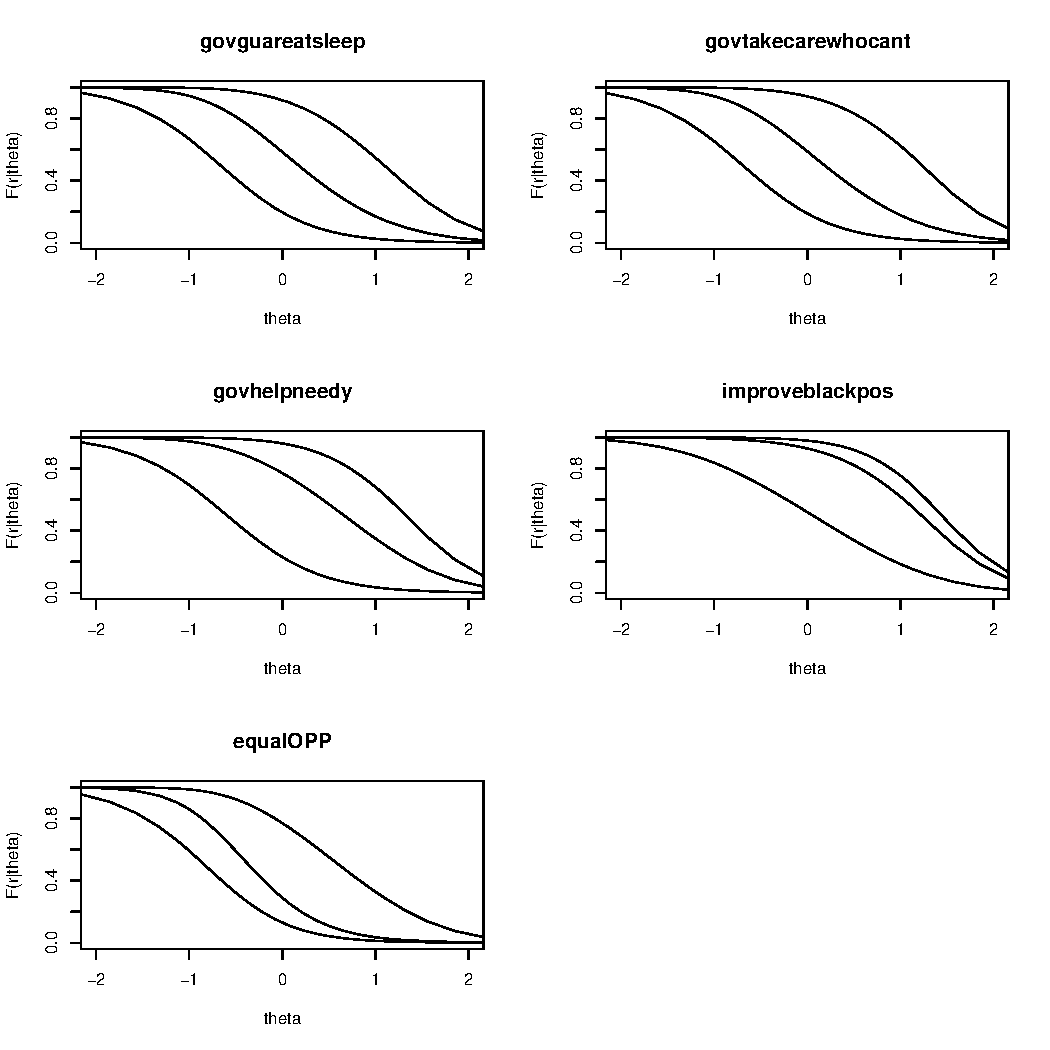
\includegraphics[width=12cm]{./graph/plotStd2.pdf}}
\end{center}
%\caption{Standard irt plot.}
%\end{figure}

Grid plots require type option. We present the second of them 
\begin{Schunk}
\begin{Sinput}
> plot(Ftab, xscale = c(-2, 2), type = "grid")
\end{Sinput}
\end{Schunk}
%\begin{figure}[hptb] 
\begin{center}
{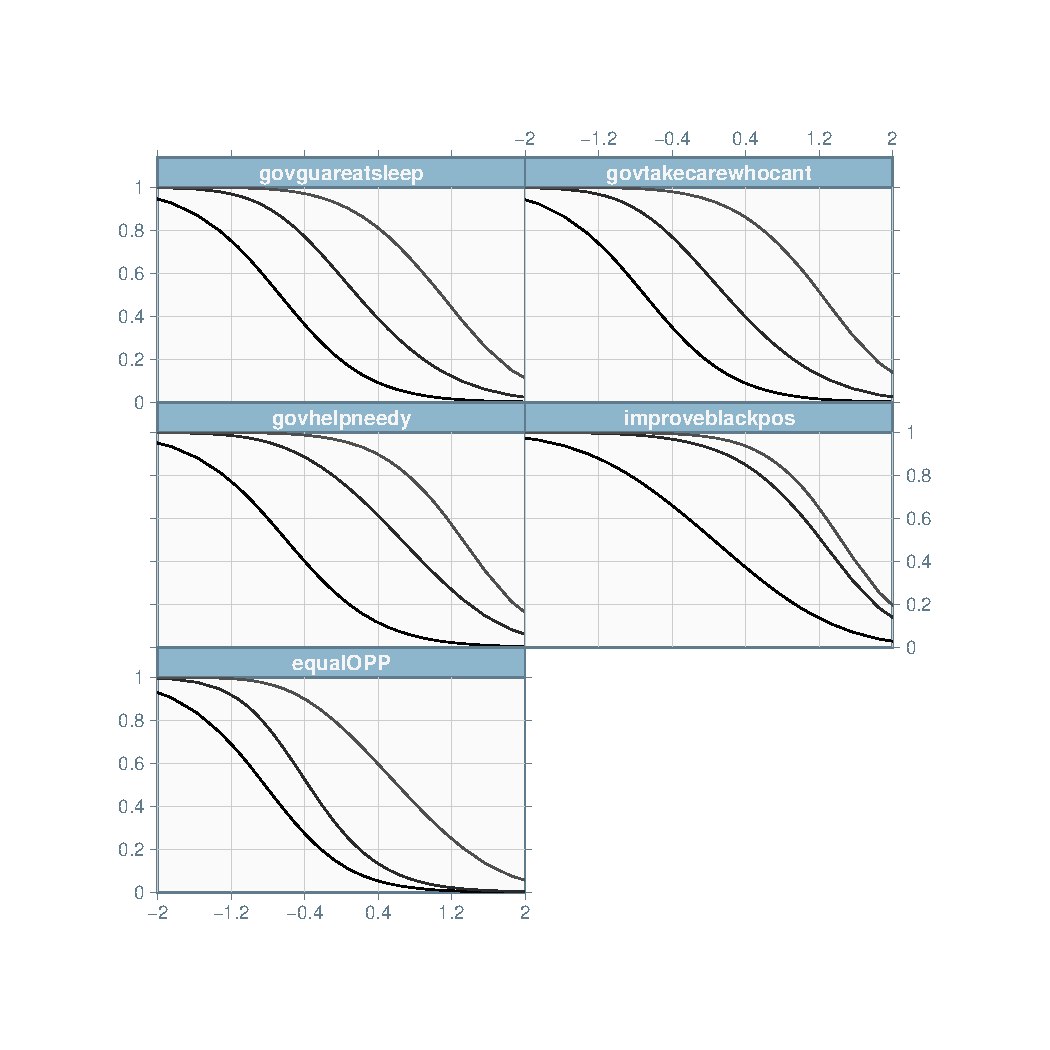
\includegraphics[width=12cm]{./graph/plotGrd2.pdf}}
\end{center}
%\caption{Standard irt plot.}
%\end{figure}

Grid graphics has also a set of color types i.e. {\it gray,black,red,blue }. They can be modified by option  {\it coltype="blue"}
\begin{Schunk}
\begin{Sinput}
> plot(Ftab, xscale = c(-3, 3), type = "grid", coltype = "blue")
\end{Sinput}
\end{Schunk}

%\begin{figure}[hptb] 
\begin{center}
{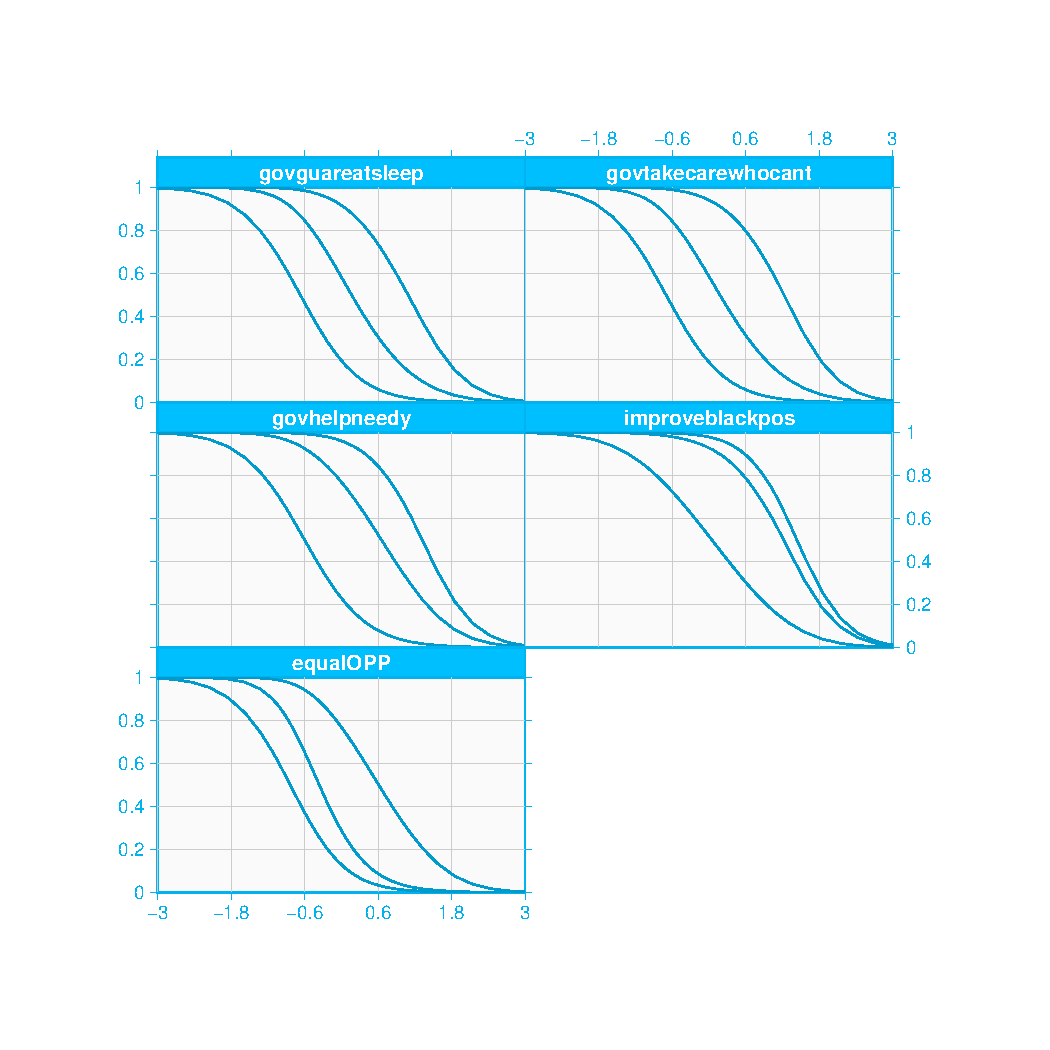
\includegraphics[width=12cm]{./graph/plotGrd2blue.pdf}}
\end{center}
%\caption{Standard irt plot.}
%\end{figure}


\section{Conclusion}
Conclusions ..

\bibliography{irtcite}
\end{document}
